%\VignetteEngine{knitr::knitr} 
%\VignetteIndexEntry{dataIrony: Exponential smoothing}

\documentclass[10pt]{article}\usepackage[]{graphicx}\usepackage[]{color}
%% maxwidth is the original width if it is less than linewidth
%% otherwise use linewidth (to make sure the graphics do not exceed the margin)
\makeatletter
\def\maxwidth{ %
  \ifdim\Gin@nat@width>\linewidth
    \linewidth
  \else
    \Gin@nat@width
  \fi
}
\makeatother

\definecolor{fgcolor}{rgb}{0.345, 0.345, 0.345}
\newcommand{\hlnum}[1]{\textcolor[rgb]{0.686,0.059,0.569}{#1}}%
\newcommand{\hlstr}[1]{\textcolor[rgb]{0.192,0.494,0.8}{#1}}%
\newcommand{\hlcom}[1]{\textcolor[rgb]{0.678,0.584,0.686}{\textit{#1}}}%
\newcommand{\hlopt}[1]{\textcolor[rgb]{0,0,0}{#1}}%
\newcommand{\hlstd}[1]{\textcolor[rgb]{0.345,0.345,0.345}{#1}}%
\newcommand{\hlkwa}[1]{\textcolor[rgb]{0.161,0.373,0.58}{\textbf{#1}}}%
\newcommand{\hlkwb}[1]{\textcolor[rgb]{0.69,0.353,0.396}{#1}}%
\newcommand{\hlkwc}[1]{\textcolor[rgb]{0.333,0.667,0.333}{#1}}%
\newcommand{\hlkwd}[1]{\textcolor[rgb]{0.737,0.353,0.396}{\textbf{#1}}}%
\let\hlipl\hlkwb

\usepackage{framed}
\makeatletter
\newenvironment{kframe}{%
 \def\at@end@of@kframe{}%
 \ifinner\ifhmode%
  \def\at@end@of@kframe{\end{minipage}}%
  \begin{minipage}{\columnwidth}%
 \fi\fi%
 \def\FrameCommand##1{\hskip\@totalleftmargin \hskip-\fboxsep
 \colorbox{shadecolor}{##1}\hskip-\fboxsep
     % There is no \\@totalrightmargin, so:
     \hskip-\linewidth \hskip-\@totalleftmargin \hskip\columnwidth}%
 \MakeFramed {\advance\hsize-\width
   \@totalleftmargin\z@ \linewidth\hsize
   \@setminipage}}%
 {\par\unskip\endMakeFramed%
 \at@end@of@kframe}
\makeatother

\definecolor{shadecolor}{rgb}{.97, .97, .97}
\definecolor{messagecolor}{rgb}{0, 0, 0}
\definecolor{warningcolor}{rgb}{1, 0, 1}
\definecolor{errorcolor}{rgb}{1, 0, 0}
\newenvironment{knitrout}{}{} % an empty environment to be redefined in TeX

\usepackage{alltt}

%\usepackage[T1]{fontenc}
%\usepackage[latin1]{inputenc}
\usepackage{boxedminipage,color,a4wide,url}
%\usepackage[utf8]{inputenc}
%\usepackage{inputenx}

\usepackage{natbib}

\input paper.bib
\def\code#1{\texttt{#1}}
\def\pkg#1{{\bf #1}}
\def\di{\pkg{dataIrony}}
\def\R{\texttt{R}}



\title{Exponential smoothing in the \di\ package}
\author{S{\o}ren H{\o}jsgaard}
%% \date{\pkg{dataIrony} version prettyVersion as of prettyDate}
\IfFileExists{upquote.sty}{\usepackage{upquote}}{}
\begin{document}

\maketitle


\def\DS{S^{[2]}}

%\setkeys{Gin}{width=0.6\textwidth}




\tableofcontents
\parindent0pt\parskip5pt

\section{Introduction}
\label{sec:introduction}

\section{Exponential smoothing}
\label{sec:expon-smooth}


\subsection{Single exponential smoothing}
\label{sec:ses}

Given is a time series $\{y_1, y_2, \dots, y_T\}$ recorded at
equidistant time points.  Single exponential smoothing (SES) of
data results in a new time series $\{S_1, S_2, \dots, S_T\}$:
\begin{displaymath}
  S_t = \alpha y_t + (1-\alpha) S_{t-1}, \quad S_1=y_1
\end{displaymath}
where $0 < \alpha < 1$.

Given data up to time $t$, the natural forecast $h$ time steps ahead is
\begin{displaymath}
  \hat y_{t+h|t} = S_t
\end{displaymath}
so the one--step--ahead forecast error is
$e_t = y_t - \hat y_{t|t-1} = y_t-S_{t-1}$.

Single exponential smoothing works well in the sense of producing
reasonable predictions if there is no clear trend in data, i.e. if
$y_t \approx a$ for all $t$.

Notice: An alternative form is:
\begin{displaymath}
  S_t = S_{t-1} + \alpha (y_t-S_{t-1}) = S_{t-1} + \alpha e_t
\end{displaymath}



\subsection{Double exponential smoothing}
\label{sec:des}


Single exponential smoothing does not work well (when it comes to producing reliable predictions) when there is a trend
in data, i.e. if $y_t \approx a + b t$.
Single exponential smoothing will be biased in the sense that
\begin{displaymath}
  y_t -S_t = b \frac{\beta}{\alpha} \mbox{ for } t\rightarrow\infty
  \mbox{ where } \beta=1-\alpha
\end{displaymath}

Hence $S_t \approx y_t - b \frac{\beta}{\alpha}$ and $y_t \approx S_t
+ b \frac{\beta}{\alpha}$ for large $t$.

If $y_t \approx a + b t$ then $S_t \approx ( a  - b
\frac{\beta}{\alpha}) + bt = \tilde a + bt$.
Therefore, if we smooth $S_t$ (i.e.\ smooth data twice) we get (by the same
argument) that
\begin{displaymath}
  S_t - \DS_t \approx b \frac{\beta}{\alpha}
\mbox{ and }
  \DS_t = (a - 2b \frac {\beta} \alpha) + bt \mbox{ for } t\rightarrow\infty
\end{displaymath}

From these considerations we therefore have
\begin{eqnarray}
  \label{eq:ses4}
  b &=& \{ S_t-\DS_t\}\frac\alpha\beta  \\
  y_t &=& S_t- b\frac{\beta}{\alpha} = S_t+(S_t-\DS_t)=2S_tt-\DS_t
\end{eqnarray}

Hence natural estimates of levels and slopes become
\begin{eqnarray}
  \label{eq:des6}
    \hat y_t   &=& S_t+\{S_t-\DS_t\}=2S_t-\DS_t\\
    \hat b_t  &=& \{S_t-\DS_t\}\frac \alpha\beta
\end{eqnarray}

Similarly, the forecasts become
\begin{equation}
  \label{eq:des7}
  \hat y_{t+h|t} = \hat y_t + \hat b_t h
\end{equation}


\section{Handling non-equidistant measurements}
\label{sec:handl-non-equid}

First consider equidistant data.  For single exponential smoothing,
the forecast error is $e_t=y_t-\hat y_{t|t-1}=y_t - S_{t-1}$. Hence
\begin{displaymath}
  S_t = S_{t-1} + \alpha e_t
\end{displaymath}
Hence, $\alpha$ is the weight attributed to the forecast error for
recordings that are one time unit apart.

For non--equidistant data we let $t_j$ denote the time of the $j$th
measurement and we have accordingly
$S_{t_j} = S_{t_{j-1}} + \alpha e_{t_j}$. Intuition suggests that the
weight attributed to the forecast error should become smaller when
$d_j = t_j - t_{j-1}$ becomes larger. Somewhat arbitrarily we handle non--equidistant measurements by
\begin{displaymath}
  S_{t_j} = S_{t_{j-1}} + w(\alpha, d_j) e_{t_j}  
\end{displaymath}
where the weight $w()$ is given by
\begin{displaymath}
  w(\alpha, d) = 1 - (1-\alpha)^{d}
\end{displaymath}


\section{Parameter estimation}
\label{sec:parameter-estimation}

For single exponential smoothing we note that minimizing
$\sum (y_t - \hat y_{t|t})^2$ will lead to $\alpha=1$ and $S_t=y_t$ so
that no smoothing takes place. Since double exponential smoothing is
simple single exponential smoothing repeated twice the same phenomenon
will appear for double exponential smoothing.


Instead we minimize (by default) the
one step ahead forecast error $\sum (y_t - \hat y_{t|t-1})^2$.

\section{Example: Nile data}
\label{example:nile}

\begin{knitrout}
\definecolor{shadecolor}{rgb}{0.969, 0.969, 0.969}\color{fgcolor}\begin{kframe}
\begin{alltt}
\hlstd{nile} \hlkwb{<-} \hlkwd{as.numeric}\hlstd{(Nile)} \hlcom{# a numeric vector}
\hlkwd{head}\hlstd{(nile)}
\end{alltt}
\begin{verbatim}
## [1] 1120 1160  963 1210 1160 1160
\end{verbatim}
\end{kframe}
\end{knitrout}

Create single and double exponential smoothing objects. When $\alpha$
is not specified, the parameter is estimated by by minimizing the
$1$--step forecasting error.
\begin{knitrout}
\definecolor{shadecolor}{rgb}{0.969, 0.969, 0.969}\color{fgcolor}\begin{kframe}
\begin{alltt}
\hlstd{ses1} \hlkwb{<-} \hlkwd{ses}\hlstd{(nile)}
\hlstd{des1} \hlkwb{<-} \hlkwd{des}\hlstd{(nile)}
\hlstd{ses1}
\end{alltt}
\begin{verbatim}
## List of 2
##  $ cls  : chr ".SES"
##  $ alpha: num 0.245
\end{verbatim}
\begin{alltt}
\hlstd{des1}
\end{alltt}
\begin{verbatim}
## List of 2
##  $ cls  : chr ".DES"
##  $ alpha: num 0.0823
\end{verbatim}
\end{kframe}
\end{knitrout}

\begin{knitrout}
\definecolor{shadecolor}{rgb}{0.969, 0.969, 0.969}\color{fgcolor}\begin{kframe}
\begin{alltt}
\hlkwd{plot}\hlstd{(nile,} \hlkwc{cex}\hlstd{=}\hlnum{.5}\hlstd{)}
\hlkwd{lines}\hlstd{(ses1,} \hlkwc{col}\hlstd{=}\hlstr{"red"}\hlstd{)}
\hlkwd{lines}\hlstd{(des1,} \hlkwc{col}\hlstd{=}\hlstr{"blue"}\hlstd{)}
\end{alltt}
\end{kframe}
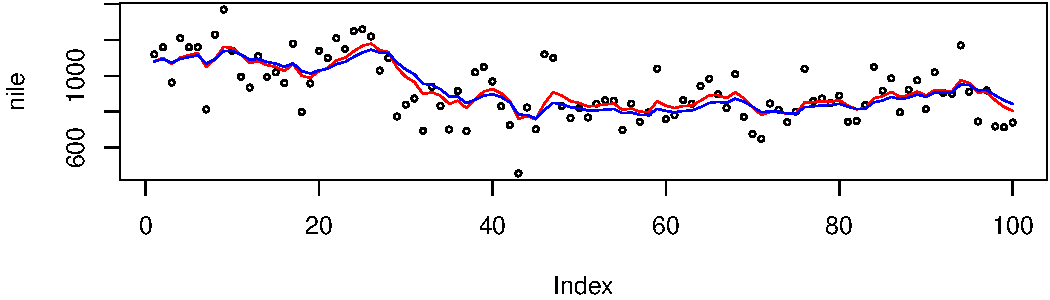
\includegraphics[width=\maxwidth]{fig/graphunnamed-chunk-6-1} 

\end{knitrout}


\begin{knitrout}
\definecolor{shadecolor}{rgb}{0.969, 0.969, 0.969}\color{fgcolor}\begin{kframe}
\begin{alltt}
\hlkwd{par}\hlstd{(}\hlkwc{mfrow}\hlstd{=}\hlkwd{c}\hlstd{(}\hlnum{2}\hlstd{,}\hlnum{1}\hlstd{))}
\hlkwd{plot}\hlstd{(ses1,} \hlkwc{cex}\hlstd{=}\hlnum{.3}\hlstd{)}
\hlstd{z} \hlkwb{<-} \hlkwd{lapply}\hlstd{(}\hlkwd{c}\hlstd{(}\hlnum{10}\hlstd{,} \hlnum{20}\hlstd{,} \hlnum{30}\hlstd{,} \hlnum{40}\hlstd{,} \hlnum{60}\hlstd{,} \hlnum{80}\hlstd{),}
       \hlkwa{function}\hlstd{(}\hlkwc{a}\hlstd{)}
           \hlkwd{lines}\hlstd{(}\hlkwd{forecast}\hlstd{(ses1,} \hlkwc{at}\hlstd{=a,} \hlkwc{h}\hlstd{=}\hlnum{1}\hlopt{:}\hlnum{10}\hlstd{),} \hlkwc{col}\hlstd{=}\hlstr{"blue"}\hlstd{,} \hlkwc{lwd}\hlstd{=}\hlnum{2}\hlstd{))}

\hlkwd{plot}\hlstd{(des1,} \hlkwc{cex}\hlstd{=}\hlnum{.3}\hlstd{)}
\hlstd{z} \hlkwb{<-} \hlkwd{lapply}\hlstd{(}\hlkwd{c}\hlstd{(}\hlnum{10}\hlstd{,} \hlnum{20}\hlstd{,} \hlnum{30}\hlstd{,} \hlnum{40}\hlstd{,} \hlnum{60}\hlstd{,} \hlnum{80}\hlstd{),}
       \hlkwa{function}\hlstd{(}\hlkwc{a}\hlstd{)}
           \hlkwd{lines}\hlstd{(}\hlkwd{forecast}\hlstd{(des1,} \hlkwc{at}\hlstd{=a,} \hlkwc{h}\hlstd{=}\hlnum{1}\hlopt{:}\hlnum{10}\hlstd{),} \hlkwc{col}\hlstd{=}\hlstr{"blue"}\hlstd{,} \hlkwc{lwd}\hlstd{=}\hlnum{2}\hlstd{))}
\end{alltt}
\end{kframe}
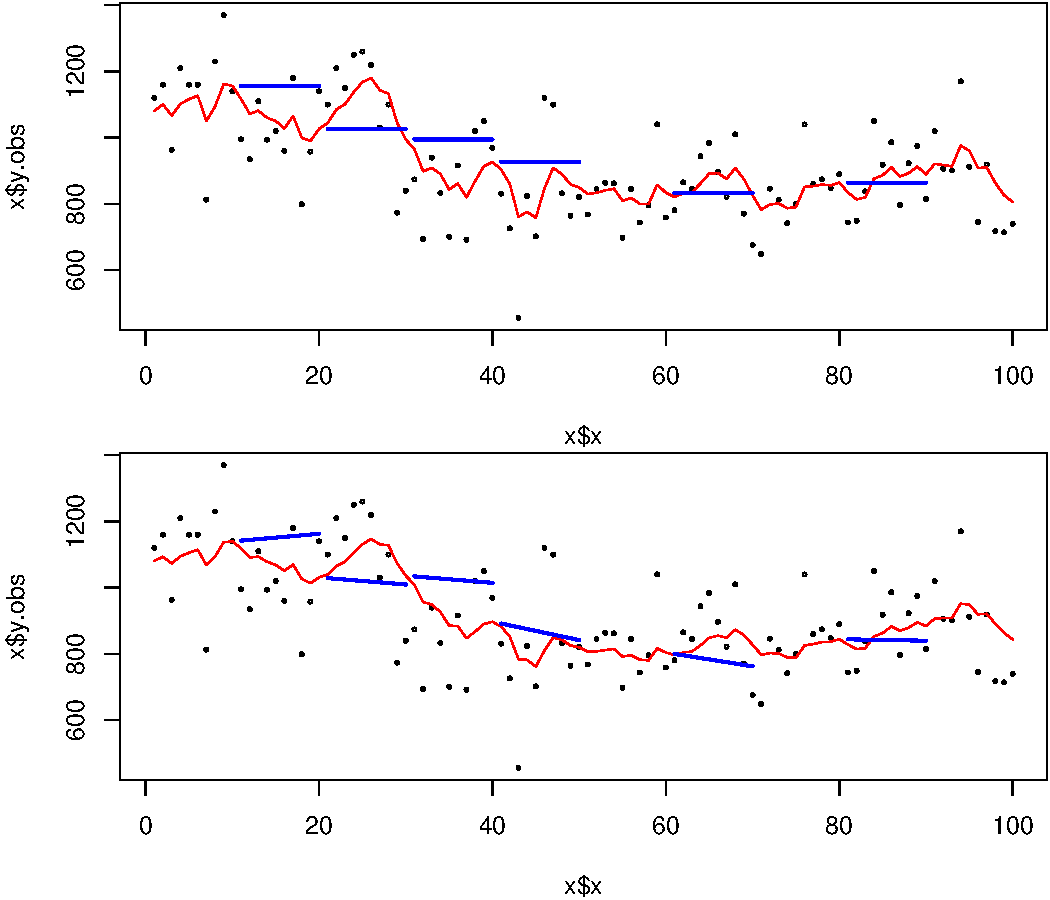
\includegraphics[width=\maxwidth]{fig/graphunnamed-chunk-7-1} 

\end{knitrout}

\section{Example: JohnsonJohnson}
\label{example:johnson}

This dataset gives the quarterly earnings (dollars) per Johnson \&
Johnson share in the period 1960-80. On the log--scale, data is approximately linear, see Fig.~\ref{fig:fig00}.

\begin{knitrout}
\definecolor{shadecolor}{rgb}{0.969, 0.969, 0.969}\color{fgcolor}\begin{kframe}
\begin{alltt}
\hlstd{y} \hlkwb{<-} \hlkwd{log10}\hlstd{(}\hlkwd{as.numeric}\hlstd{(JohnsonJohnson))}
\hlkwd{par}\hlstd{(}\hlkwc{mfrow}\hlstd{=}\hlkwd{c}\hlstd{(}\hlnum{1}\hlstd{,}\hlnum{2}\hlstd{))}
\hlkwd{plot}\hlstd{(JohnsonJohnson);} \hlkwd{plot}\hlstd{(y,} \hlkwc{cex}\hlstd{=}\hlnum{.5}\hlstd{)}
\end{alltt}
\end{kframe}\begin{figure}
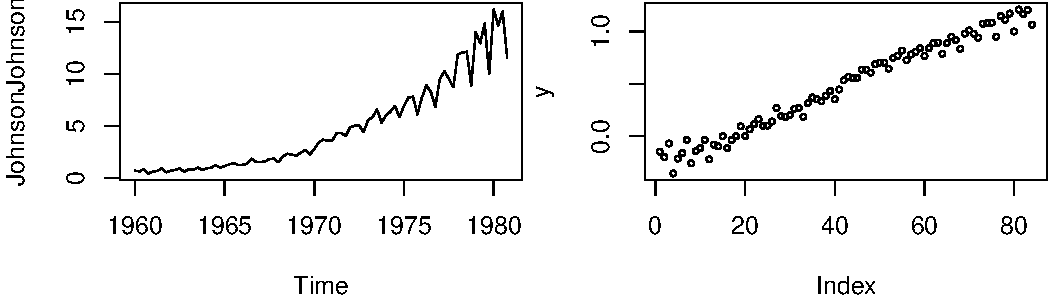
\includegraphics[width=\maxwidth]{fig/graphfig00-1} \caption[bla]{bla}\label{fig:fig00}
\end{figure}


\end{knitrout}


The bias in SES is clear if a small value of $\alpha$ is chosen, whereas DES quickly captures the structure in data, see Fig.~\ref{fig:fig01}.

\begin{knitrout}
\definecolor{shadecolor}{rgb}{0.969, 0.969, 0.969}\color{fgcolor}\begin{kframe}
\begin{alltt}
\hlstd{ses1} \hlkwb{<-} \hlkwd{ses}\hlstd{(y,} \hlkwc{alpha}\hlstd{=}\hlnum{.1}\hlstd{,} \hlkwc{fit}\hlstd{=}\hlnum{FALSE}\hlstd{)}
\hlstd{des1} \hlkwb{<-} \hlkwd{des}\hlstd{(y,} \hlkwc{alpha}\hlstd{=}\hlnum{.1}\hlstd{,} \hlkwc{fit}\hlstd{=}\hlnum{FALSE}\hlstd{)}
\hlstd{ses1}
\end{alltt}
\begin{verbatim}
## List of 2
##  $ cls  : chr ".SES"
##  $ alpha: num 0.1
\end{verbatim}
\begin{alltt}
\hlstd{des1}
\end{alltt}
\begin{verbatim}
## List of 2
##  $ cls  : chr ".DES"
##  $ alpha: num 0.1
\end{verbatim}
\end{kframe}
\end{knitrout}

\begin{knitrout}
\definecolor{shadecolor}{rgb}{0.969, 0.969, 0.969}\color{fgcolor}\begin{figure}
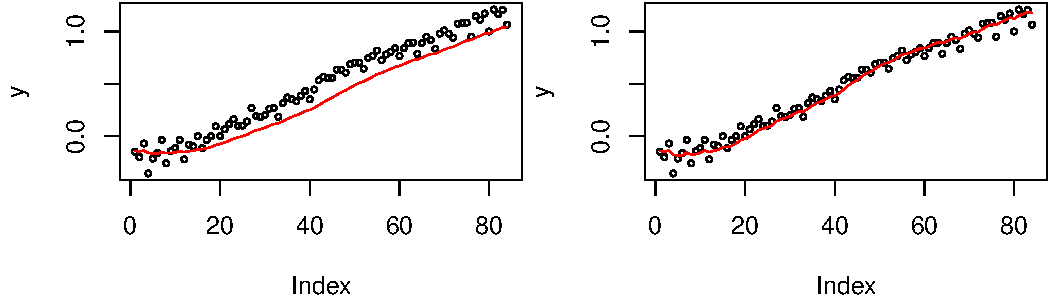
\includegraphics[width=\maxwidth]{fig/graphfig01-1} \caption[bla]{bla}\label{fig:fig01}
\end{figure}


\end{knitrout}

When fitting $\alpha$ to data, the smoothed values fit better to data,
but the predictions of SES are bad because of the linear trend in
data, cfr.\ Fig.~\ref{fig:fig02}.

\begin{knitrout}
\definecolor{shadecolor}{rgb}{0.969, 0.969, 0.969}\color{fgcolor}\begin{kframe}
\begin{alltt}
\hlstd{ses1} \hlkwb{<-} \hlkwd{ses}\hlstd{(y)}
\hlstd{des1} \hlkwb{<-} \hlkwd{des}\hlstd{(y)}
\hlstd{ses1}
\end{alltt}
\begin{verbatim}
## List of 2
##  $ cls  : chr ".SES"
##  $ alpha: num 0.502
\end{verbatim}
\begin{alltt}
\hlstd{des1}
\end{alltt}
\begin{verbatim}
## List of 2
##  $ cls  : chr ".DES"
##  $ alpha: num 0.16
\end{verbatim}
\end{kframe}
\end{knitrout}

\begin{knitrout}
\definecolor{shadecolor}{rgb}{0.969, 0.969, 0.969}\color{fgcolor}\begin{figure}
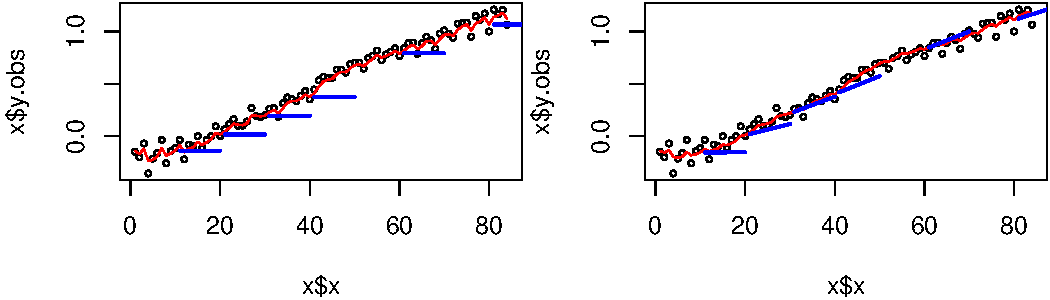
\includegraphics[width=\maxwidth]{fig/graphfig02-1} \caption[bla]{bla}\label{fig:fig02}
\end{figure}


\end{knitrout}




\bibliographystyle{apalike}
\bibliography{paper}




\end{document}













%% \section{Example: Seatbelts}
%% \label{sec:seatbelts}

%% <<>>=
%% sb <- as.data.frame(Seatbelts)
%% head(sb)
%% y <- sb$DriversKilled
%% plot(y)
%% @ 

%% <<small.mar=T>>=
%% ses1 <- ses(y)
%% ses1
%% par(mfrow=c(1,2))
%% plot(y, cex=.5); 
%% lines(ses1, xlab='', col="red") 
%% plot(residuals(ses1), cex=.5); abline(h=0)
%% @ %def








%% \section{Example}
%% \label{sec:example}

%% << >>= 

%% yvar <- aggregate(co2)
%% tvar <- seq_along(yvar)
%% f1 <- ses(yvar, tvar)
%% f2 <- des(yvar, tvar)
%% at <- 1 + seq(0, 35, by=5)

%% plot(f1)
%% forecast_lines(f1, at=at, ahead=0:5, col='red', lwd=3)
%% forecast_lines(f2, at=at, ahead=0:5, col='blue', lwd=3)

%% @



%% Add more noise to data: 
%% << >>= 
%% yvar2 <- yvar + rnorm(length(yvar), sd=40)
%% f1 <- ses(yvar2, tvar)
%% f2 <- des(yvar2, tvar)

%% plot(f1)
%% at <- 1 + seq(0, 35, by=5)
%% forecast_lines(f1, at=at, ahead=0:5, col='red', lwd=3)
%% forecast_lines(f2, at=at, ahead=0:5, col='blue', lwd=3)
%%@







